\documentclass[a4paper,11pt]{article}
\usepackage[utf8]{inputenc}
\usepackage{amsmath}
\usepackage{multicol}
\usepackage{booktabs}
\usepackage{longtable}
%opening
\title{Graph-based pattern sampling for solve-repair heuristic}
\author{}

\setlength{\topmargin}{-2.1cm}
\setlength{\textwidth}{15.8cm}
\setlength{\textheight}{26.3cm}
\setlength{\oddsidemargin}{-0.1cm}
\setlength{\evensidemargin}{-0.1cm}

\def\II{{\mathcal{I}}}
\def\TT{{\mathcal{T}}}
\def\KK{{\mathcal{K}}}
\def\JJ{{\mathcal{J}}}

\usepackage{graphicx}
\usepackage{amssymb}
\usepackage{chngcntr}
\usepackage[linesnumbered,ruled,vlined]{algorithm2e}
\usepackage{tikz}
\usetikzlibrary{arrows.meta}
\tikzset{%
  >={Latex[width=2mm,length=2mm]},
  % Specifications for style of nodes:
            base/.style = {rectangle, rounded corners, draw=black,
                           minimum width=4cm, minimum height=1cm,
                           text centered, font=\sffamily},
  activityStarts/.style = {base, fill=blue!30},
       startstop/.style = {base, fill=red!30},
    subproblem/.style = {base, fill=green!30},
         master/.style = {base, minimum width=2.5cm, fill=orange!15,
                           font=\ttfamily},
}

\counterwithin*{equation}{section}
\counterwithin*{equation}{subsection}

\begin{document}

\maketitle

\section{Introduction}
  \label{sec:model}

  The purpose of this document is to present the implemented idea of a general solve-repair technique using random and efficient pattern sampling at each iteration to solve the Military Flight and Maintenance Problem.

  The first section is a description of the input data. Then the master problem is presented. The pattern definition, representation and sampling follows. Lastly, several alternatives to subproblems are described.

\subsection{Pattern}

  We call pattern to a feasible combination of missions assignments and checks for aircraft $i$ between the beginning of period $t$ and the end of period $t^\prime$.

\section{Input data}

    \subsection{Basic sets}

        \begin{tabular}{p{15mm}p{140mm}}
            $i \in \mathcal{I}$     &  aircraft. \\
            $t \in \mathcal{T}$     &  time periods included in the planning horizon. \\
            $j \in \mathcal{J}$     &  missions. \\
            $y \in \mathcal{Y}$     &  types of mission or aircraft. \\
            $k \in \mathcal{K}$     &  clusters of aircraft that share exactly the same functionality. \\
            $p \in \mathcal{P}$     &  all possible patterns to assign to any aircraft. \\
        \end{tabular}

    \subsection{Mission parameters}

        \begin{tabular}{p{15mm}p{125mm}p{15mm}}
            $R_j$             & number of aircraft required by mission $j$. & aircraft. \\
        \end{tabular}

    \subsection{Maintenance parameters}

        \begin{tabular}{p{15mm}p{125mm}p{15mm}}
            $C^{max}$         & maximum number of simultaneous checks. & aircraft. \\
        \end{tabular}

    \subsection{Fleet parameters}

        \begin{tabular}{p{15mm}p{125mm}p{15mm}}
            $N_t$               & number of aircraft known to be in maintenance in period $t$. & aircraft. \\
            $N^{Clust}_{kt}$    & number of aircraft in cluster $k$ known to be in maintenance in period $t$. & aircraft. \\
            $A^{Clust}_{kt}$    & maximum number of aircraft in cluster $k$ that can be simultaneously in maintenance in period $t$. & aircraft. \\
            $H^{Clust}_{kt}$    & minimum number of total remaining flight time for cluster $k$ at period $t$. & hours. \\
            $Y_i$               & type $y \in \mathcal{Y}$ for aircraft $j$. & type. \\
            $Rft_{itp}$           & remaining flight time for aircraft $i \in \mathcal{I}$ at the end of period $t \in \mathcal{T}$ if assigned pattern $p \in \mathcal{PI}_i$. & hours. \\
        \end{tabular}

    \subsection{Parametric sets}

        \begin{tabular}{p{15mm}p{140mm}}
          $t \in \mathcal{TJ}_j$     &  time periods $t \in \mathcal{T}$ in which mission $j$ is active. \\
          $j \in \mathcal{JT}_t$    &  missions $j \in \mathcal{J}$ to be realized in period $t$. \\
          $i \in \mathcal{IK}_k$     &  aircraft $i \in \mathcal{I}$ that are included in cluster $k$. One aircraft can belong to more than one cluster. \\
          $j \in \mathcal{JI}_i$     &  missions $j \in \mathcal{J}$ for which aircraft $i$ can be used. \\
          $i \in \mathcal{A}^{Init}_j$  & aircraft $i \in \mathcal{I}$ that have mission $j$ pre-assigned in the previous period to the start of the planning horizon. \\
          $p \in \mathcal{PI}_i$     &  patterns $p \in \mathcal{P}$ that are available for aircraft $i$. \\
          $p \in \mathcal{PT}^{M}_{it}$     &  patterns $p \in \mathcal{PI}_i$ where aircraft $i$ is in maintenance in period $t \in \mathcal{T}$. \\
          $p \in \mathcal{PT}^{J}_{itj}$     &  patterns $p \in \mathcal{PI}_i$ where aircraft $i i \in \mathcal{IJ}_j$ is assigned to mission $j \in \mathcal{J}$ in period $t \in \mathcal{T}$. \\
        \end{tabular}

    \subsection{Interval deviation and objective function parameters}

       \begin{tabular}{p{15mm}p{105mm}p{15mm}}
            $P\hspace{-0.5mm}A_s$   & penalty cost for violating serviceability constraint in interval $s$. & [$\frac{penalty}{aircraft.period}$] \\
            $P\hspace{-0.5mm}H_s$   & penalty cost for violating sustainability constraint in interval $s$. & [$\frac{penalty}{hour-period}$] \\
            $PC_s$   & penalty cost for violating capacity constraint in interval $s$. & [$\frac{penalty}{aircraft.period}$]\\
            $PM_p$    & reward per period for the start of each check in patter $p$. & [$\frac{penalty}{aircraft.period}$]\\
            $U\hspace{-0.5mm}A_s$   & maximum deviation for violating the serviceability limit in interval $s$. & [aircraft] \\
            $U\hspace{-0.5mm}H_s$   & maximum deviation for violating the sustainability limit in interval $s$. & [hours] \\
            $U\hspace{-0.5mm}C_s$   & maximum deviation for violating the maintenance capacity limit in interval $s$. & [aircraft] \\
        \end{tabular}

\section{General logic and master problem}


  The master problem is used to do the following tasks at each iteration.

  \begin{enumerate}
    \item Find good candidates of time window ($\mathcal{T}_{c}$) and aircrafts ($\mathcal{I}_{c}$) to repair.
    \item Call the subproblem to obtain a new solution.
    \item Decide whether to accept or not the new solution.
  \end{enumerate}

  The initial solution ($c=0$) consists of calling the subproblem with a time window the size of the planning horizon ($\mathcal{T}_{0} = \mathcal{T}$) and the complete set of aircraft ($\mathcal{I}_{0} = \mathcal{I}$).

  \begin{tikzpicture}[node distance=1.5cm,
    every node/.style={fill=white, font=\sffamily}, align=center]
  % Specification of nodes (position, etc.)
    \node (start)             [activityStarts]              {Start};
    \node (initSol)     [startstop, below of=start]          {Initial solution};
    \node (maybeStop)      [master, below of=initSol]   {Reached time limit \\or max iterations?};
    \node (Stop)      [activityStarts, right of=maybeStop, xshift=4cm]   {End};
    \node (objFunc)      [master, below of=maybeStop]   {Get objective};
    \node (bestSol)      [master, below of=objFunc]   {Update best solution};
    \node (prevSol)      [master, below of=bestSol]   {Update previous solution};
    \node (getErrors)      [master, below of=prevSol]   {Get errors $e$};
    \node (getCandidate)     [master, below of=getErrors]   {Find candidate $\mathcal{T}_{c}$, $\mathcal{I}_{c}$};
    \node (samplePatterns)      [subproblem, below of=getCandidate]
                                                        {Sample patterns};
    \node (decidePatterns)      [subproblem, below of=samplePatterns]
                                                                  {Decide patterns};
    \node (applyPatterns)       [subproblem, below of=decidePatterns]
                                                                   {Apply patterns};
    % \node (ActivityDestroyed) [startstop, below of=onDestroyBlock]
    %                                                   {Activity is shut down};     
    % Specification of lines between nodes specified above
    % with aditional nodes for description 
    \draw[->]             (start) -- (initSol);
    \draw[->]     (initSol) -- (maybeStop);
    \draw[->]     (maybeStop) -- (Stop);
    \draw[->]     (maybeStop) -- (objFunc);
    \draw[->]     (objFunc) -- (bestSol);
    \draw[->]      (bestSol) -- (prevSol);
    \draw[->]      (prevSol) -- (getErrors);
    \draw[->]      (getErrors) -- (getCandidate);
    \draw[->]     (getCandidate) -- (samplePatterns);
    \draw[->]      (samplePatterns) -- (decidePatterns);
    \draw[->]      (decidePatterns) -- (applyPatterns);
    % \draw[->]       (applyPatterns) -- node {The activity is shut down by
    %                                  user or system} (onDestroyBlock);
    % \draw[->]    (onDestroyBlock) -- (ActivityDestroyed);
    % \draw[->]      (decidePatterns) -| node(priorityXMemory)
    %                                  {higher priority $\rightarrow$ more memory}
    %                                  (ActivityEnds);
    % \draw           (applyPatterns) -| (priorityXMemory);
    % \draw[->]     (ActivityEnds)  |- node [yshift=-2cm, text width=3.1cm]
                                      % {User navigates back to the activity}
                                      % (initSol);
    % \draw[->]      (applyPatterns.east) -- (objFunc.east);
  \draw[->] (applyPatterns.west) -- ++(-2.6,0) -- ++(0,10) -- ++(0,2) --                
     (maybeStop.west);
  \end{tikzpicture}

\section{Pattern generation}

  \subsection{Graph representation}

    A Directed Acyclic Graph (DAG) is created for each aircraft. Each node in the graph represents the state of the aircraft at a specific period in time. Thus, the node is represented by a unique combination of: 

        \begin{tabular}{p{10mm}p{115mm}}
          $rft$    &  remaining flight time. \\
          $rct$    &  remaining calendar time. \\
          $t^s$    &  assignment starting period. \\
          $t^f$    &  assignment ending period. \\
          $y$      &  assignment type (check, mission, empty). \\
          $j$      &  assignment value (in the case of missions, the mission; in the case of checks, 'M'; else it is empty). \\
        \end{tabular}

    Each outbound neighbor of a node represents a state the aircraft can have on the immediately next (future) period. This guarantees that the graph will never have any cycles, since we only consider neighbors that are in the future of the current node and, as a consequence, have not been observed yet.


    The graph in Figure \ref{fig:graph_resource1} represents the set of transitions for an individual aircraft in an horizon of 10 periods. A pattern consists of a single unique path that starts at the source node at the extreme left (named "2017-12" in the Figure) and end at the sink node at the extreme right (named "2018-11" in the Figure).

    \begin{figure}
        \centering
        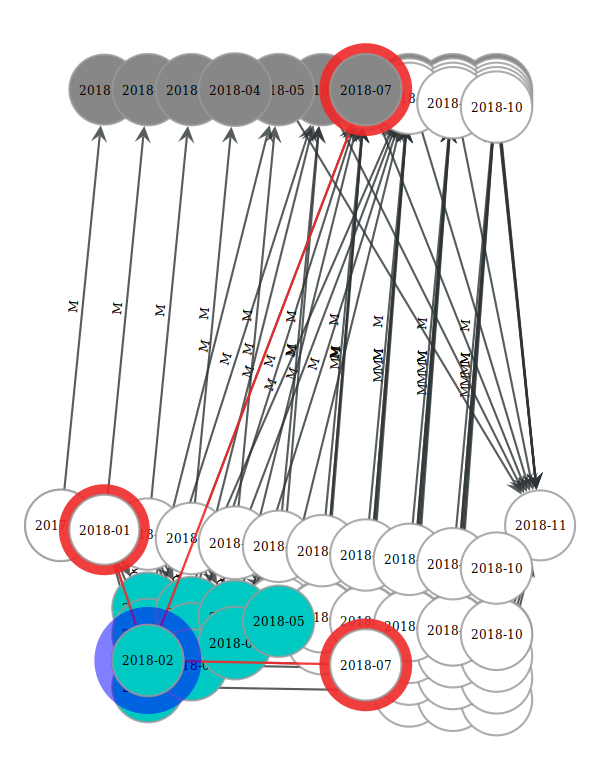
\includegraphics[height=0.7 \linewidth]{example_graph_1.png}
        \caption{DAG representing the transitions of a single aircraft. Each node represents a combination of an assignment at a given time. Nodes are plotted with time in the horizontal axis and the remaining flight time of the aircraft in the vertical axis. White nodes represent an empty assignment (of duration 1). Gray nodes represent a check (of duration 6). Finally, colored nodes represent a mission assignment (the assignment's duration can vary). A example node (circled in blue) is selected and their neighbors (circled in red) are shown: one inbound to the left and two outbound to the right. The selected node consists of an assignment to mission "O1" between periods "2018-02" and "2018-06".} \label{fig:graph_resource1}
    \end{figure}

  \subsection{Graph creation}

    In order to generate a graph from an aircraft, an exhaustive exploration of all possible states for a given aircraft needs to be done. This exploration starts in a node we will call source, where we apply a depth-first search (DFS), looking at each step for all the immediately consecutive neighbors of the node.

    Algorithm \ref{algo:graph-building} shows the procedure executed to create the graph for every aircraft. The logic of $get\_neighbors$ is described in Function \ref{algo:node-neighbors}. TODO: finish describing the $get\_neighbors$ function.

    \begin{algorithm}
    \DontPrintSemicolon
    \SetKwData{node}{$n$}
    \SetKwData{remaining}{$rem$}
    \SetKwData{graph}{$G$}
    \SetKwData{fix}{$f$}
    \KwData{\\$n$: current node. \\$rem$: list of remaining nodes to visit. \\$f$: fix initial states.}
    \KwResult{\\$G$: graph, represented by a mapping between nodes and a list of their neighbors.}
    \BlankLine
    \Begin{
      $\node \leftarrow get\_source\_node()$\;
      $\remaining \leftarrow [\node]$\;
      \If{$|\fix| > 0$}{
        $\remaining \leftarrow \graph[\node] \leftarrow get\_fixed\_nodes(\fix)$\;
      }
      \While{$|\remaining| > 0$}{
        $\node \leftarrow \remaining.pop()$\;
        \If{$\node \notin \graph$}{
          $\graph[\node] \leftarrow get\_neighbors(\node)$\;
          $\remaining.Add(\graph[\node]) $\;
        }
      }
      $\graph \leftarrow add\_artificial\_end\_nodes(\graph)$\label{algo:artificial}\;
    }
    \caption{Depth-first search to populate states graph}\label{algo:graph-building}
    \end{algorithm}

    \begin{algorithm}
    \DontPrintSemicolon
    \SetKwData{node}{$n$}
    \KwData{\\$n$: current node.}
    \BlankLine
    \Begin{
      \If{$\node.end ==last\_period$}{
        $return [get\_sink\_node()]$\;
      }
      $\node.Get\_maint\_neighbors()$\;
      $\node.Get\_mission\_neighbors()$\;
      $\node.Get\_nothing\_neighbors()$\;
    }
    \caption{Get neighbors from node}\label{algo:node-neighbors}
    \end{algorithm}

  \subsection{Path extraction}

    Given a Graph $G(X,V)$, we want to generate all paths from any node $X_1 \in X$ to node $X_2 \in X$. This can be achieved using a DFS and a maximum length cutoff for the search. In our case the maximum length cutoff is trivial to calculate since it equals the number of periods between the two nodes, given that a valid path never overlaps assignments at the same time.

    We obtain those two nodes in the graph, given an existing feasible solution and the time window $\mathcal{T}_{c}$.
    For the first node $X_1$ we do the following. Let $t_{init}$ be the first period in time window $\mathcal{T}_{c}$, we calculate the state of the aircraft $i \in \mathcal{I}_{c}$ in period $t_{init}$. In the case the assignment is an empty assignment, the state will be directly calculated using $rft=rft_i$, $rct=rct_i$, $t^s=t^f=t_{init}$, $y=2$, $j=''$. In the case the assignment is a check or mission assignment, one needs to find the initial period ($t^\prime_{init}$) and the end period ($t^{\prime\prime}_{init}$) for the assignment update the rest accordingly: $rft=rft_i$, $rct=rct_i$, $t^s=t^\prime_{init}$, $t^f=t^{\prime\prime}_{init}$, $y=1$, $j='1'$ if the assignment is mission '1'.

    For the second node $X_2$ this process needs to be modified somewhat since we do not want to fix the $rct$ and $rft$ of the end node. This implies creating several artificial nodes that have $rft=-1$ and $rct=-1$ and connecting all the other nodes that share $t^s, t^f, y, j$ to these nodes. This is done in Line \ref{algo:artificial} of Algorithm \ref{algo:graph-building}. Let $t_{end}$ be the last period in time window $\mathcal{T}_{c}$. We then calculate the end node like so: $rft=-1$, $rct=-1$, $t^s=t^\prime_{end}$, $t^f=t^{\prime\prime}_{end}$, $y=0$, $j='M'$ for the case the assignment at the end is a check.

    Using the example in figure \ref{fig:graph_resource1}, there exist 5 unique paths that start in the selected node in blue. Table \ref{tab:pattern_enumeration} shows all possible patterns for that aircraft that start in that node and finish in the sink.

    \begin{longtable}{llllllllll}
\toprule
0 &  O1 &  O1 &  O1 &  O1 &  O1 &  M &  M &  M &  M \\
1 &  O1 &  O1 &  O1 &  O1 &  O1 &    &  M &  M &  M \\
2 &  O1 &  O1 &  O1 &  O1 &  O1 &    &    &  M &  M \\
3 &  O1 &  O1 &  O1 &  O1 &  O1 &    &    &    &  M \\
4 &  O1 &  O1 &  O1 &  O1 &  O1 &    &    &    &    \\
\end{longtable}


  \subsection{Sampling paths}

    The previous procedure can be trivially modified so it renders a maximum number of paths at each time, by stopping the DFS process after a number of paths is returned. This, nevertheless, results in a extremely biased sampling of the paths since, by construction, the DFS guarantees that consecutive paths share most of the path. In addition to this, by default, most DFS implementations use the same sequence of choices given the same graph. This approach is, thus, limited.

    The first question that arises is how to take unbiased samples of paths in a graph, in between two nodes. This is possible and can be done in a DAG by first pre-calculating the number of paths that pass through each node in their trip from $X_1$ to $X_2$. This last operation can be done in $\mathcal{O}(V)$, where $V$ is the number of edges in between the two nodes. Then, we use this information to sample one neighbor at each node when iterating from $X_1$. This implies not doing a DFS but starting each path at $X_1$.

    The second question that arises is how to take biased samples of paths in a graph, by giving more probability to paths that are similar to the paths we are looking for (i.e., have nodes that are more useful for the solution). This implies having information about the paths we are looking for, which we do from the Master (e.g., the same information we use to determine where to repair: the number of errors in the solution). Doing this avoids having to generate too many samples to get a good solution.

\section{Subproblem}

  The subproblem is a pattern-aircraft assignment problem. 
  In each iteration $c$, it takes as input the following:

  \begin{enumerate}
    \item A range of consecutive dates $\mathcal{T}_{c} \subset \mathcal{T}$ (time window).
    \item A set of aircraft $\mathcal{I}_{c} \subset \mathcal{I}$.
  \end{enumerate}
  
  The main steps this algorithm does are:

  \begin{enumerate}
    \item For each aircraft $i \in \mathcal{I}_{c}$, sample $N$ feasible patterns. Each pattern starts at the beginning of $\mathcal{T}_{c}$ and ends at the end of $\mathcal{T}_{c}$.
    \item For each aircraft, decide one pattern from those $N$ sampled patterns.
    \item Apply each pattern to each aircraft.
  \end{enumerate}

  Step 2 can be accomplished in more than one way. Section \ref{model} shows the use of a mathematical model, Section \ref{grasp} shows the use of a heuristic solution.

  \subsection{Assignment model}
    \label{model}

    Given a subset of samples for each aircraft, we solve an assignment problem using a mixed-integer lineal programming solver. The model is explained below.

    \subsubsection{Variables}

      The following decision variables control the assignment of missions and checks to aircraft.

      \begin{tabular}{p{8mm}p{147mm}}
          $a_{ip}$ &  =1 if aircraft $i$ uses pattern $p$. \\  
      \end{tabular}

      Auxiliary variables control the status of each aircraft or group of aircraft.

      \begin{tabular}{p{8mm}p{147mm}}
          $e^{A}_{kts}$ & Continuous, positive. Elastic variable for serviceability constraint (\ref{eq:serviceability-cluster}). \\
          $e^{H}_{kts}$ & Continuous, positive. Elastic variable for sustainability constraint (\ref{eq:sustainability-cluster}). \\
          $e^{C}_{ts}$ & Continuous, positive. Elastic variable for capacity constraint (\ref{eq:capacity1}). \\
          $e^{J}_{jts}$ & Continuous, positive. Elastic variable for mission aircraft needs constraint (\ref{eq:missionres}). \\
      \end{tabular}

    \subsubsection{Objective function and constraints}
      Objective (\ref{eq:objective1}) minimizes the deviations on elastic constraints while penalizing patterns with earlier checks.

      \begin{align}
          & \text{Min}\; 
          \sum_{\substack{
                  k \in \mathcal{K}, \\ t \in \mathcal{T}, \\ s \in \mathcal{S}
                  }
              } PA_s e^{A}_{kts} 
          + \sum_{\substack{
                  k \in \mathcal{K}, \\ t \in \mathcal{T}, \\ s \in \mathcal{S}
                  } 
              } PH_s e^{H}_{kts}
          + \sum_{t \in \mathcal{T}, s \in \mathcal{S}} PC_s e^{C}_{ts}
          - \sum_{i \in \mathcal{I}, p \in \mathcal{PI}_i} PM_p a_{ip}
          \label{eq:objective1}
      \end{align}

      The following constraints are used in the model:
      \begin{align}
          % maximum capacity1:
          & \sum_{\substack{i \in \mathcal{I}, \\ p \in \mathcal{PT}^{M}_{it}}} a_{ip} + N_t \leq C^{max} + \sum_{s \in \mathcal{S}} e^{C}_{ts}
                  & t \in \mathcal{T} \label{eq:capacity1}\\
          % min assignments:
          & \sum_{\substack{i \in \mathcal{IJ}_j, \\ p \in \mathcal{PT}^{J}_{itj}}} a_{ip} + \sum_{s \in \mathcal{S}} e^{J}_{jts} \geq R_j
                  & j \in \mathcal{J}, t \in \mathcal{TJ}_j  \label{eq:missionres}\\
      \end{align}

      Maintenance capacity is controlled by (\ref{eq:capacity1}). The aircraft requirements of missions are defined by (\ref{eq:missionres}).

      \begin{align}
         & \sum_{\substack{i \in \mathcal{IK}_k, \\ p \in \mathcal{PT}^{M}_{it}}} a_{ip} + N^{Clust}_{kt} \leq A^{Clust}_{kt} + \sum_{s \in \mathcal{S}} e^{A}_{kts}
              & k \in \mathcal{K}, t \in \mathcal{T} \label{eq:serviceability-cluster}\\
         & \sum_{\substack{i \in \mathcal{IK}_k, \\ p \in \mathcal{PI}_i}} Rft_{itp} a_{ip} \geq H^{Clust}_{kt} - \sum_{s \in \mathcal{S}} e^{H}_{kts}
              & k \in \mathcal{K}, t \in \mathcal{T} \label{eq:sustainability-cluster}
      \end{align}

      Constraints (\ref{eq:serviceability-cluster}) guarantee a minimum serviceability of aircraft for each cluster $k$. A cluster is defined by the largest group of aircraft that is required exclusively for at least one mission. 
      Constraints (\ref{eq:sustainability-cluster}) ensure there is a minimum amount of remaining flight hours for each cluster $k$.

      \begin{align}
          & \sum_{p \in \mathcal{PI}_i} a_{ip} =  1 
            & i \in \mathcal{I}\label{eq:num_maint} \\
      \end{align}

      Constraints (\ref{eq:num_maint}) assure each aircraft will have only one assigned pattern.

  \subsection{GRASP heuristic}
    \label{grasp}

    Given a subset of samples for each aircraft, we iteratively choose one pattern for each aircraft. The probability of each pattern to be included depends on the improvement of the pattern to the objective function in its current status. Algorithm \ref{algo:sample_heur} shows this logic.

    \begin{algorithm}
    \DontPrintSemicolon
    \SetKwData{sol}{$x$}
    \SetKwData{pattern}{$p$}
    \SetKwData{patterns}{$\mathcal{P}$}
    \KwData{\\\sol: current solution. \\\patterns: set of patterns for aircraft $i$ in time window $\mathcal{T}_{c}$. \\\pattern: sampled pattern.}
    \BlankLine
    \Begin{
      \For{$i \in \mathcal{I}_{c}$}{
        $\patterns \leftarrow get\_patterns(i, \mathcal{T}_{c})$\;
        $\pattern \leftarrow sample\_pattern(\sol, \patterns)$\;
        $\sol.Apply(\pattern)$\;
      }
    }
    \caption{An heuristic to sample patterns iteratively}\label{algo:sample_heur}
    \end{algorithm}

  \subsection{Graph heuristic}
    \label{graphHeur}

    This heuristic is a variant of the previous one. Instead of obtaining a previous sample before re-sampling, we obtain directly one pattern per Aircraft. We do this by giving weights to each edge on the graph and using those weights to sample iteratively the resulting pattern for the aircraft.

    Another alternative is to generate random edges and do a shortest\_path.


\end{document}